\chapter{Introduction}
In this report we propose a design of the $\delta$-GOC-Ledger \cite{delta-goc-ledger-heisch} over a byzantine fault tolerant log, which is largely based upon the design of 2P-BFT-Log proposed by Lavoie \cite{2p-bft-log}. In doing so, we discovered the need for a new message type (see section \ref{sec:choices}).

In our design, we introduced to the best of our knowledge novel invariants (see section \ref{sec:invariants}). These invariants are: \var{d1} to \var{d7}, \var{M8} and \var{F1} to \var{F4}. To accommodate the new message type, we also adjusted the invariants \var{M3} and \var{M4} from the design of 2P-BFT-Log.

Additionally, we designed and implemented an algorithm that we argue verifies all of these invariants except for \var{F4} on a given the set of messages. The implementation was done over Git, where we used a more efficient encoding of the data that needs to be tracked by the $\delta$-GOC-Ledger by previous approaches \cite{delta-goc-ledger-heisch}.
The performance of this algorithm and our efficient encoding was evaluated on a basic benchmark of randomly generated transactions (see section \ref{sec:evaluation}).
This algorithm was then optimized (see section \ref{sec:summary-cache}) with what we argue is an optimization that improves the asymptotic running time of the algorithm (see section \ref{sec:results:perf-baseline}) in the case of the basic benchmark.

The implementation of the algorithm and source code of this report can be found on the following repository: \url{https://github.com/p-vf/verify-goc-ledger}

\chapter{Background}
In this section, relevant background to the concepts in this project are provided. \\

\section{Append-only logs as Hash-Graphs}
An Append-only log is a distributed data structure that allows participants to share messages between each other. This is done by having each participant have a totally ordered set of messages that gets replicated to the other participants. This can be implemented using hash-graphs, where each message contains the hash of the previous message (if there is any) of the same author. By using a cryptographic hash, we know the messages cannot have been tampered with, as hash-collisions are computationally hard to find. By cryptographically signing the messages we can guarantee that the correct author created the message.

However one problem that arises is that an adversary E can create two messages that are concurrent to each other by referencing the same previous message and distributing each of those messages to different parts of the network. Once the correct participants have replicated these messages, this results in the set of messages belonging to E no longer being totally ordered, breaking the design of naive implementations of append-only logs. In this scenario we say that the log of E is \emph{forked} and E is an \emph{equivocator} \cite{blocklace-crdt}.

If the append-only log is implemented as a hash-graph, dependencies between messages of different authors can be modelled by including a set of hashes into a message which represent its immediate dependencies. Such dependencies are necessary to order messages by causality, i.e. if there is a hash in the dependencies of message A belonging to message B, we know the message B must have been created before the message A (see happens-before relationship, eqn. \ref{eqn:happens-before}).

\section{2P-BFT-Log}
2P-BFT-Log is a design that implements an append-only log data structure and behaves just like one as long as there are no forks. As soon as there is evidence of a fork in a log, any further messages of the corresponding author are ignored \cite{2p-bft-log}. If there is no fork in a given log, the log is said to be in the \emph{growing phase}, otherwise it is in the \emph{shrinking phase}.

\subsection{Messages}
The design of 2P-BFT-Log consists of several parts. First of all, each message has certain contents, each of which is called a field. The fields of a message and their corresponding type and meaning are listed in Table \ref{tab:2p-bft-log-msg-content}.

\begin{table}
    \begin{tabular}{|l|l|p{5cm}|}
    \hline
    \textbf{Field} & \textbf{Type} & \textbf{Meaning}\\
    \hline
    $M_\emph{author}$ & String (Public Key) & author of the message \\
    $M_\emph{prev}$ & MsgId or $\bot$ & previous message from same author, $\bot$ (null) if none.\\
    $M_\emph{deps}$ & Set of MsgId & State of logs from other authors on which the message depends\\
    $M_\emph{payload}$ & String & Content of message, in our case representing either an account update or a byzantine acknowledgement (see sections \ref{sec:account-as-str} and \ref{sec:ack-as-str} respectively) \\
    $M_\emph{signature}$ & String & Signature of the concatenation of the previous fields using the private key corresponding to $M_\emph{author}$.\\
    $M_\emph{date}$ & Date & Date the message was created at \\
    \hline
    \end{tabular}
    \caption{Contents of a message according to the design of 2P-BFT-Log}
    \label{tab:2p-bft-log-msg-content}
\end{table}

To identify and reference messages, the function $\msgId$ is used.
It is the hash derived from the concatenation of the contents of the message, i.e.
\[
    \msgId(M) \definedas H(M_\emph{author} \oplus M_\emph{prev} \oplus M_\emph{deps} \oplus M_\emph{payload} \oplus M_\emph{signature} \oplus M_\emph{date})
\]
where $H$ is a cryptographic hash function.

Additionally there are some relevant relations that are defined on messages.
The first one is the \emph{happens-before} relationship and is defined as:
\begin{equation}
    M \rightsquigarrow M' \definedas \begin{cases}
        M = M'_\emph{prev} = \bot \\
        \msgId(M) = M'\emph{prev} \\
        \msgId(M) \in M'\emph{deps} \\
        \exists M'' : M \rightsquigarrow M'' \rightsquigarrow M'
    \end{cases}
    \label{eqn:happens-before}
\end{equation}

Additionally, the author-specific happens-before relationship is defined as
\begin{equation}
    M \happensbeforelog M' \definedas \begin{cases}
        M = M'_\emph{prev} = \bot \\
        \msgId(M) = M'\emph{prev} \\
        \exists M'' : M \happensbeforelog M'' \happensbeforelog M'
    \end{cases}
    \label{eqn:happens-before-author}
\end{equation}


Based on the happens-before relationship, the partial order on messages ($\le_\mathcal{M}$) is defined:
\[
    M \le_\mathcal{M} M' \definedas M = M' \lor M \rightsquigarrow M'
\]

If neither $M$ or $M'$ is smaller than the other, they are called concurrent ($\parallel_\mathcal{M}$).
\[
    M \parallel_\mathcal{M} M' \definedas M {\nleq_\mathcal{M}} M' \land M' {\nleq_\mathcal{M}} M
\]

We define the strict causal history of message $M$ as the messages that happened before message $M$:
\[
    \mathcal H_<(M) \definedas \{M' : M' \rightsquigarrow M\}
\]
Additionally we define the causal history of message $M$ as
\[
    \mathcal H_\le(M) \definedas \{M' : M' \le_\mathcal{M} M\}
\]

If $S$ is a set of messages, the (strict) causal history of $S$ is overloaded and means the (strict) causal history of all the messages in $S$ combined.
\[
    \mathcal H_r(S) \definedas \bigcup_{M \in S}\mathcal H_r(M)
\]


\section{\(\delta\)-GOC-Ledger}

The Grow-Only-Counter-Ledger (GOC-Ledger) is a consensus-free data structure that implements a ledger designed to be used to track transactions of crypto-tokens. A ledger needs to track which author owns how many tokens, to be able to check how many tokens they are able to spend in subsequent transactions. An account $A$ is the unit of data that keeps track of this information. Multiple such accounts from different authors form the state of the ledger. More concretely, a ledger $L$ is a mapping from authors to their corresponding account.

In the case of the GOC-Ledger, this is realized by introducing 5 fields: $A_\emph{author}$ which is the author of this account, $A_\uparrow$ and $A_\downarrow$ which represent the number of created/destroyed tokens respectively, $A_\rightarrow$ and $A_\leftarrow$ which represent the number of given/received tokens respectively. $A_\uparrow$ and $A_\downarrow$ are simple grow-only counters whereas $A_\rightarrow$ and $A_\leftarrow$ are mappings from author names to grow-only counters, which represent the number of tokens $A_\emph{author}$ has given to or acknowledged from the other author respectively.

For ease of writing, the notation $S_*$ is defined to be the domain of definition of a mapping $S$. E.g. if $L$ is a ledger, $L_*$ denotes the set of authors that have an account in this ledger.

To get the balance of an account, we can compute \[\balance(A) \definedas A_\uparrow + \left(\sum_{a \in A_{\leftarrow*}} A_\leftarrow[a]\right) - A_\downarrow - \left(\sum_{a \in A_{\rightarrow*}} A_\rightarrow[a]\right)\].
Additionally there is a merge operation with which accounts can be merged. This merge function is only defined on accounts of the same author and returns the account that contains the maximal values of all the grow only counters in both of the accounts and adds all the grow-only counters that are only in one of the two accounts. I.e. for accounts $A$ and $B$, the merged account $C = A \sqcup B$ is defined as:
\begin{align*}
    C_\emph{author} &= A_\emph{author} = B_\emph{author}\\
    C_\uparrow &= \max\{A_\uparrow, B_\uparrow\}\\
    C_\downarrow &= \max\{A_\downarrow, B_\downarrow\}\\
    C_\rightarrow &= \{x \mapsto A_\rightarrow[x] \mid x \in A_{\rightarrow*} \setminus B_{\rightarrow*}\} \\
    &\quad \cup \{x \mapsto B_\rightarrow[x] \mid x \in B_{\rightarrow*} \setminus A_{\rightarrow*}\} \\
    &\quad \cup \{x \mapsto \max\{A_\rightarrow[x], B_\rightarrow[x]\} \mid x \in B_{\rightarrow*} \cap A_{\rightarrow*}\}\\
    C_\leftarrow &= \ldots \text{(analogous to $C_\rightarrow$)}\\
\end{align*}


Furthermore, there is also a merge operation on a ledger and an account. The ledger and an account get merged by merging the account with the corresponding account in the ledger if the author is present and if not, adding the account to the ledger. Formally, if we have a ledger $L$ and account $A$, $L' = L \sqcup A$ is defined as:

\begin{align*}
    L'[A_\emph{author}] &=\begin{cases} L[A_\emph{author}] \sqcup A & \text{ if } A_\emph{author} \in L_* \\
            A & \text{ otherwise}
        \end{cases}\\
    L'[x] &= L[x] \quad \text{for any $x \in L_*$ with $x \ne A_\emph{author}$}
\end{align*}

Additionally, we define a repeated merge operation over a set of accounts $\mathcal A = \{A_1, \ldots, A_n\}$ as the ledger after applying the account updates:
\[
\bigsqcup_{A \in \mathcal A} A \definedas \left(\left(\ldots\left(\left(\emptyset \sqcup A_1\right) \sqcup A_2\right) \sqcup\ldots\right)\sqcup A_{n-1}\right)\sqcup A_n
\]


\subsection{Delta Accounts}
To store the state of the ledger more efficiently with regards to space, only the grow-only counters that have changed have to be stored. This is done via delta accounts as proposed by Heisch \cite{delta-goc-ledger-heisch}. A delta account $A^\delta$ has the same fields as a normal account, just that the fields $A^\delta_\uparrow$ and $A^\delta_\downarrow$ evaluate to the default value $0$ if they are not stored and the fields $A^\delta_\rightarrow$ and $A^\delta_\leftarrow$ evaluate to $\emptyset$ when not stored. When merging delta accounts, one can use the merge operation on normal accounts, evaluating missing fields to their default value.


\chapter{Design}

\section{Definitions}

$\textsc{Signed}$ of message $M$ is the predicate that is true iff $M_\emph{signature}$ is a valid signature belonging to $M_\emph{author}$.

$\textsc{Signed}_A(\mathcal M)$ is defined as the set of messages in $\mathcal M$ that are created and signed correctly by author $A$, formally:
\[
    \textsc{Signed}_A(\mathcal M) \definedas \{M \in \mathcal M \mid \textsc{Signed}(M) \land M_\emph{author} = A\}
\]

A fork proof is a set of messages which all have the same previous message. We define fork proofs as a predicate $\forkproof$ over a set of messages $S$.
\[
    \forkproof(S) \definedas
    \bigwedge_{M, M' \in S} \left(
        \begin{aligned}
            &M_\emph{prev} = M'_\emph{prev}
            \land M_\emph{author} = M'_\emph{author} \\
            &\land \textsc{Signed}(M)
            \land \textsc{Signed}(M')
        \end{aligned}
    \right)
\]

The function \var{deps} of message $M$ is defined as the messages in its immediate dependencies.
\[\var{deps}(M) \definedas \{M' \mid \msgId(M') \in M_\emph{deps}\}\]

Similarly, the function \var{prev} of $M$ denotes its previous message.
\[\var{prev}(M) \definedas \begin{cases}
    M' &\text{ if there exists } M' : \msgId(M') = M_\emph{prev}\\
    \bot & \text{ otherwise}
\end{cases} \]

A message $M$ in our design can have one of two types; either it has the type account (denoted \var{ACCOUNT}) or it has the type byzantine acknowledgement (denoted \var{BYZ\_ACK}). The type is encoded within its payload and retrieved with $\msgType(M)$. The roles of these message types is specified in section \ref{sec:choices}. The function $\acc$ is the function that retrieves the account fields encoded in $M_\emph{payload}$, the author identifier from $M_\emph{author}$ (i.e. $(\acc(M))_\emph{author} = M_\emph{author}$), and is only defined if $\msgType(M) = \var{ACCOUNT}$.

The set $\max_A(\mathcal M)$ is the set of message ids belonging to maximal messages in the set of messages $\mathcal M$ that were created by author $A$, when looking at the author-specific happens-before relationship ($\happensbeforelog$).
\[
    \max_A(\mathcal M) \definedas \{\msgId(M) \mid M \in \textsc{Signed}_A(\mathcal M) \land \forall M' \in \textsc{Signed}_A(\mathcal M) : M \not\happensbeforelog M'\}
\]

Since there are multiple authors that we need to track during verification, we combine this information in a frontier. A frontier is a map of author names to a set of messages and is defined over a set of messages $\mathcal M$, written $F(\mathcal M)$.
\begin{equation}
    \label{eqn:frontier}
    F(\mathcal M) \definedas \{A \mapsto \max_A(\mathcal M) \mid \exists M \in \mathcal M : A = M_\emph{author} \land \textsc{Signed}(M)\}
\end{equation}

\section{Choices}
\label{sec:choices}
In our design we made some choices. To save space, we only keep track of the necessary dependencies in a message, meaning only the participants of a transaction are allowed to be in the dependencies of the corresponding message. A consequence of this is that if this is the only way to replicate messages, proof of byzantine behaviour can only be shared if a transaction with actual tokens is made. This prompted us to add a second message type, the \var{BYZ\_ACK} message (a normal transaction has message type \var{ACCOUNT}).
This message type is there to point out to other replicas that some of the participants behave badly, and to prevent colluders from being able to keep ignoring evidence of a fork.

\section{Detecting Byzantine Behaviour}
For specifying invariants related to byzantine behaviour, it is necessary to define what we consider byzantine behaviour. This is mostly based on the Blocklace paper by Almeida et al. \cite{blocklace-crdt}, but was adapted to the design of 2P-BFT-Log.
The function \var{byz} of a set of messages $S$ is the set of authors exhibiting byzantine behaviour in the set $S$ and is defined as follows:
\begin{align*}
    \var{byz}(S) \definedas \{a \mid\,&\exists M \in S : \\
    &a = M_\emph{author}\\
    &\land \textsc{Signed}(M)\\
    &\land (\\
    &\qquad \exists M' \in S : \forkproof(\{M, M'\}) \\
    % &\qquad \lor \lnot \var{wellFormed}(M)\\
    &\qquad \lor \lnot \var{valid}(M) \\
    &)\}
\end{align*}

Where $\var{valid}$ is a predicate that is true iff the message is syntactically well formed (see section \ref{sec:syntax-of-msgs}), and further invariants hold for the message specified in section \ref{sec:invariants}. It is important to note that our design of the predicate $\var{valid}$ does not follow the convention proposed in the design of the Blocklace paper that messages from known byzantine actors are ignored as (see section \ref{sec:invariants-delta-a} for justification).

\section{Invariants}
\label{sec:invariants}

\subsection{Invariants on message \(M\) and corresponding delta account}
\label{sec:invariants-delta-a}
The following invariants only apply, if $\msgType(M) = \var{ACCOUNT}$.
Let $L_\emph{before}$ be the state of the ledger before update $\deltacc{A}$ was performed. Formally, this can be described as
\begin{equation}
    L_\emph{before} = \bigsqcup_{M' \in H_\emph{acc}} \acc(M')
    \label{eqn:l-before-def}
\end{equation}
where $H_\emph{acc} = \{M' \in \mathcal H_<(M) \mid \msgType(M') = \var{ACCOUNT} \land \var{valid}(M')\}$ is the set of all delta accounts in the strict causal history of $M$.

Since we merge account states no matter if the corresponding authors exhibited byzantine behaviour, this means that double spending is not prevented nor handled correctly: if a double spending happens, tokens get created out of thin air by the equivocator. This leads to byzantine processes being able to generate an arbitrary number of tokens. However fixing this issue is more involved: if we simply ignore messages that come from byzantine processes, correct replicas that received money from such byzantine replicas lose tokens, which might lead to a negative balance which is not allowed under normal circumstances. An economical design that handles double spending in some way, preventing correct replicas from losing tokens due to invalidated messages is required to fix this issue but is outside the scope of this project.

For this project, we assume that the predicate \var{valid} may depend on messages in the causal history from known equivocators to avoid negative balance in valid account messages. This is in contrast to the design described in the Blocklace paper, where the valid predicate may only depend on messages in the causal history from authors that don't exhibit byzantine behaviour. This means that if the balance of an account is negative, this can only have been caused by either a) the author overspending tokens or b) there being a fork in the causal history of the same account, where the double spending happened. In case a) the message is invalid and in case b) the message can also be viewed as invalid, because it is guaranteed to be created by a byzantine process, which means no message $M$ with $\msgType(M) = \var{ACCOUNT}$ should ever reference it anyway. So in either case, a negative balance invalidates a message.

$L_\textit{after}$ represents the ledger after $\deltacc A$ has been applied to $L_\textit{before}$, so $L_\emph{after} = L_\emph{before} \sqcup \deltacc{A}$.

Further, let $A^\delta = \acc(M)$ be the delta account stored in $M$.

The invariant \var{d1} ensures that there are no unnecessary GOCs stored in $A^\delta$. An unnecessary GOC is a GOC that doesn't increase the corresponding GOC in $L_\emph{before}$ when merged with it. This means each GOC in $A^\delta$ must be positive and strictly greater than the previous value in $L_\emph{before}$ if it exists.
\begin{invariant}{\var{d1}}
    (minimal):
    $A^\delta_\uparrow \neq 0 \neq A^\delta_\downarrow$ holds and for all $n \in \text{image}(A^\delta_\rightarrow)\cup \text{image}(A^\delta_\rightarrow)$, $n > 0$ holds.
    If $M_\emph{author} \in (L_\emph{before})_*$, then all of the following holds, where $A_\emph{old} = L_\emph{before}[M_\emph{author}]$:
    \begin{itemize}
        \item if $A^\delta_\uparrow \neq 0$, then $(A_\emph{old})_\uparrow < A^\delta_\uparrow$,
        \item if $A^\delta_\downarrow \neq 0$, then $(A_\emph{old})_\downarrow < A^\delta_\downarrow$,
        \item for all $a \in A^\delta_{\rightarrow*} \cap (A_\emph{old})_{\rightarrow*}$, $(A_\emph{old})_{\rightarrow}[a] < A^\delta_{\rightarrow}[a]$ holds,
        \item for all $a \in A^\delta_{\leftarrow*} \cap (A_\emph{old})_{\leftarrow*}$, $(A_\emph{old})_{\leftarrow}[a] < A^\delta_{\leftarrow}[a]$ holds.
    \end{itemize}
\end{invariant}
The invariant \var{d5} ensures that at least one of the fields $\deltacc A_\rightarrow$, $\deltacc A_\leftarrow$, $\deltacc A_\uparrow$, $\deltacc A_\downarrow$ is defined, except if the message contains the first delta account.
\begin{invariant}{\var{d5}}
    (account not empty): If $M_\emph{author} \in (L_\emph{before})_*$, then
    $A^\delta_\uparrow \neq 0 \lor A^\delta_\downarrow \neq 0 \lor A^\delta_\rightarrow \neq \emptyset \lor A^\delta_\leftarrow \neq \emptyset$ holds.
\end{invariant}
The invariant \var{d2} ensures that accounts don't have negative balance.
\begin{invariant}{\var{d2}}
    (non-negative balance): The constraint $\balance(L_\textit{after}[M_\emph{author}]) \ge 0$ holds.
\end{invariant}
The invariant \var{d3} ensures that all the tokens that were acknowledged, where actually given to the account before $M$.
\begin{invariant}{\var{d3}}
    (valid acknowledgements) If $\deltacc A_\leftarrow$ is non-empty, the constraint $\deltacc A_\leftarrow[x] \le (L_\textit{before}[x])_\rightarrow[M_\emph{author}]$ must hold for all $x \in \deltacc A_{\leftarrow*}$.
\end{invariant}
Invariant \var{d4} ensures that only replicas that are permitted can create tokens. For the purposes of this report, we define the set $\var{Creators}$ which contains all the authors that are allowed to create tokens.
\begin{invariant}{\var{d4}}
    (valid creator) If $\deltacc A_\uparrow \neq 0$, $\deltacc A_\emph{author} \in \var{Creators}$.
\end{invariant}

We want the dependencies that are necessary to track the origins of a transaction. However, we don't want unnecessarily many dependencies. For example if $\acc(M)$ is a transaction between authors \var{A}, \var{B} and \var{C}, where \var{A} is the creator of the message, we want exactly one message in the immediate dependencies $M_\emph{deps}$ created by author \var{B} and exactly one created by \var{C}.

A message $M'$ is relevant to message $M$ iff message $M$ acknowledges tokens from $M_\emph{author}$.
\begin{invariant}{\var{d6}}
    (relevant dependencies): all the dependencies of $M$ are relevant, i.e. for all $M' \in \var{deps}(M)$ it holds that $M'_\textit{author} \in \acc(M)_{\leftarrow *}$.
\end{invariant}
One thing to note here is that only the authors in the field $\acc(M)_{\leftarrow *}$ get checked. If there is an author in $\acc(M)_{\rightarrow *}$ that doesn't exist or has exhibited byzantine behaviour, this is semantically the same as if the tokens given to that non-existent author were destroyed (meaning $\acc(M)_\downarrow$ being increased by this amount) and is always allowed.

Furthermore, we need to check that there is exactly one dependency for each author mentioned in the acked field. That there is at most one dependency per author is covered by the invariant \var{M4}.
\begin{invariant}{\var{d7}}
    (necessary dependencies): for any author $a \in \acc(M)_{\leftarrow *}$, there exists a message $M'$ with $M'_\textit{author} = a$ and $\msgId(M') \in M_\textit{deps}$
\end{invariant}

\subsection{Invariants on Message \(M\) inherited from 2P-BFT-Log}
\begin{enumerate}
    \item [\var{M1}] \emph{(single previous dependency)}: either $M_\textit{prev} = \bot$ or $M_\textit{prev} = \msgId(M'): M'$ exists and is valid.
    \item [\var{M2}] \emph{(single author)}: if $M_\textit{prev} = \msgId(M')$ then $M'_\textit{author} = M_\textit{author}$.
    \item [\var{M3}] \emph{(valid external dependencies)}: for all $\textit{\var{\var{msgId}}} \in M_\textit{deps}$, there exists a $M'$ such that $\msgId(M') = \var{msgId}$ and $M'_\textit{author} \neq M_\textit{author}$. If $\msgType(M) = \var{ACCOUNT}$, $\var{valid}(M')$ must be true.
    \item [\var{M4}] \emph{(single author dependencies)}: for any possible \textit{author} not equal to $M_\textit{author}$, and any $M' \in \var{deps}(M)$, the following must hold: If $\msgType(M) = \var{ACCOUNT}$, then there must be at most one $M'$ such that $M'_\textit{author} = \textit{author}$.
    \item [\var{M5}] \emph{(self-certifying)}: $M_\textit{signature}$ is consistent with $M_\textit{author}$, i.e. $\textsc{Signed}(M)$ is true.
    \item [\var{M6}] \emph{(acyclic)}: $M_\textit{prev}$ does not reference a successor of $M$, i.e. ($M_\textit{prev} \neq M' : M \stackrel{\textit{log}}{\rightsquigarrow} M'$).
    \item [\var{M7}] \emph{(monotonic dependencies)}: For all $M'$ with $M \stackrel{log}{\rightsquigarrow} M'$, the following must hold: for all $(D, D') \in \var{deps}(M) \times \var{deps}(M')$ with $D_\textit{author} = D'_\textit{author}$, $D \le_\mathcal M D'$ holds.
    \item [\var{M8}] \emph{(non-decreasing dates)}: if $M_\emph{prev} \ne \bot$, $(\var{prev}(M))_\textit{date} \leq M_\textit{date}$ must hold
\end{enumerate}
We adjusted M3 to ignore validity when $\msgType(M) = \var{BYZ\_ACK}$, as byzantine acknowledgements are allowed to have invalid messages as dependencies (see section \ref{sec:invariants-byz}). Furthermore, we adjusted M4 to only apply if $\msgType(M) = \var{ACCOUNT}$, because if the message is a byzantine acknowledgement, we want to be able to have two dependencies from the same author in case of a fork. We also added the invariant \var{M8} to allow for sorting the messages of one author by date.
% Validity properties if log $L$ is in growing phase:
% \begin{enumerate}
%     \item [CL1] \emph{(no forks)}: $L_\textit{forks} = \emptyset$.
%     \item [CL2] \emph{(valid last message)}: if $L_\textit{last} = M \neq \bot$ then $M$ is valid.
%     \item [CL3] \emph{(consistent previous author)}: if $L_\textit{last} \neq \bot$ then $L_\textit{author} = (L_\textit{last})_\textit{author}$.
% \end{enumerate}
% Validity properties if log $L$ is in shrinking phase:
% \begin{enumerate}
%     \item [FL1] \emph{(non-empty forks)}: $L_\textit{forks} \neq \emptyset$.
%     \item [FL2] \emph{(valid last message)}: same as CL2.
%     \item [FL3] \emph{(consistent previous author)}: same as CL3.
%     \item [FL4] \emph{(valid forks)}: for all $M \in L_\textit{forks}$, $M$ is valid.
%     \item [FL5] \emph{(consistent fork author)}: for all $M \in L_\textit{forks}$, $L_\textit{author} = M_\textit{author}$ and if $L_\textit{last} \neq \bot$ then $L_\textit{author} = (L_\textit{last})_\textit{author}$.
%     \item [FL6] \emph{(valid proof)}: if $M \in L_\textit{forks}$ then $\exists M' \in L_\textit{forks}$ such that $M \neq M'$ and $M_\textit{prev} = M'_\textit{prev}$.
%     \item [FL7] \emph{(consistent proof)}: for all $M \in L_\textit{forks}$, $L_\textit{last} = M_\textit{prev}$.
% \end{enumerate}

\subsection{Invariants related to Byzantine Behaviour}
\label{sec:invariants-byz}
We want to ensure that authors don't make any transactions with an author that has created messages that exhibit byzantine behaviour. To enforce this, we check that any author that is part of the transaction must not exhibit byzantine behaviour in the set of messages known to author at the time (denoted $\mathcal H_\leq(M)$). This invariant is only enforced on messages of type \var{ACCOUNT}.
\begin{invariant}{\var{F1}}
    \emph{(No transactions after byzantine message)}:\\
    If $\msgType(M) = \var{ACCOUNT}$, then the following must hold: for any author $a \in \var{byz}(\mathcal H_<(M))$, there must be no message $M' \in \var{deps}(M)$ with $M'_\emph{author} = a$.
\end{invariant}

We also want to ensure that participants don't make transactions with authors that haven't acknowledged the byzantine behaviour present in the message graph. This means that if there is byzantine behaviour in the set of messages known to a message, all its immediate dependencies must know about this (see invariant \var{F2}). An exclusion is made for byzantine acknowledgement messages, as - by design - they cannot satisfy this criteria.
\begin{invariant}{\var{F2}}
    \emph{(acknowledgement before transaction)}:\\
    If $\msgType(M) = \var{ACCOUNT}$ then the following must hold for any message $M' \in \var{deps}(M)$:
    $$\var{byz}(\mathcal H_<(M)) = \var{byz}(\mathcal H_\leq(M'))$$.
\end{invariant}

To ensure that byzantine acknowledgement messages only have necessary immediate dependencies (in the same sense as before), we check that if any of the messages in the immediate dependencies were to be removed, the set of byzantine authors would shrink (see invariant \var{F4}).

\begin{invariant}{\var{F3}}
    \emph{(necessary dependencies of acknowledgement)}:\\
    If $\msgType(M) = \var{BYZ\_ACK}$ then for all $M'\in \var{deps}(M)$, the condition $$\var{byz}(\mathcal H_\le((\var{deps}(M) \cup \{\var{prev}(M)\}) \setminus \{M'\}) ) \subset \var{byz}(\mathcal H_<(M))$$ must hold.
\end{invariant}

The invariant \var{F4} ensures that additionally, any message that is in the dependencies must be a minimal message that makes its author byzantine.

\begin{invariant}{\var{F4}}
    \emph{(minimal dependencies of acknowledgement)}:\\
    If $\msgType(M) = \var{BYZ\_ACK}$ then for all $M'\in \var{deps}(M)$, the condition $$\var{byz}(\mathcal H_<(M) \setminus \{M'\}) \subset \var{byz}(\mathcal H_<(M))$$ must hold.
\end{invariant}

Our algorithm does not verify the invariant \var{F4}, but \var{F3} which is quite similar, but easier to verify. In \var{F3}, there is no requirement for minimality of the message $M'$. This means that any of the messages that get added to the causal history by $M'$ must make a new author byzantine, not just the message $M'$.

If we only verify \var{F3} this allows colluders to pollute the causal history with arbitrarily many messages after a fork in a log. To show this, we can take a look at an example; If $E$ is a byzantine node and $C$ its colluder, where $E$ has forked their log and created many messages after this on either end. A colluder can then include any of these messages in the causal history with a byzantine acknowledgement message. So long as this acknowledgement is the first message that acknowledges the byzantine behaviour of $E$, this message is labeled as valid by \var{F3}. If we look at \var{F4}, we see that such behaviour would not be allowed. $C$ would have to acknowledge the first message that proves $E$'s byzantine behaviour.

\section{Syntax of Messages}
\label{sec:syntax-of-msgs}
For a message $M$ to be well formed, $M_\emph{payload}$ must contain a valid string that encodes either a delta account or a byzantine acknowledgement. The requirements on the syntax are implemented in a predicate $\var{wellFormed}$ which is true iff its argument is a syntactically well formed message according to the implementation specific encoding that is used. How this is implemented in our case can be seen in Section~\ref{sec:payload-syntax}.

\section{Algorithm for Verification}
To verify a replica, its messages are visited in an arbitrary ascending topological order according to the relation $\rightsquigarrow$, meaning if $M \rightsquigarrow M'$, $M$ must be visited before $M'$. Each message gets checked for the invariants and if it is valid, it is added to the set of valid message ids $F_\emph{valid}$.
%\footnote{If memory is a concern, the immediate predecessors of $M$ can be removed from $F_\emph{valid}$ and the check if a message $M'$ has been validated before becomes is there a $\var{msgId} \in F_\emph{valid}$ with $M'  \le_\mathcal{M} C_\emph{msg}[\var{msgId}]$. This makes $F_\emph{valid}$ a sort of frontier of valid messages.}

\begin{algorithm}[ht]
\caption{Basic structure of the verifying algorithm}
\begin{algorithmic}[1]
\Function{VerifyReplica}{set of messages $\mathcal M$}
    \State $F_\emph{valid} \gets \emptyset$ \Comment{The set of ids corresponding to valid messages}
    \State $C_\emph{msg} \gets \emptyset$ \Comment{A mapping from message ids to messages}
    \ForAll{$M \in \mathcal{M}$ in a topological order}
        \State $C_\emph{msg}[\msgId(M)] \gets M$
        \If{$\Call{VerifyMessage}{M, C_\emph{msg}, F_\emph{valid}}$}
            \State $F_\emph{valid} \gets F_\emph{valid} \cup \{\msgId(M)\}$ \Comment{add $M$ as valid message}
            % \State $F_\emph{valid} \gets F_\emph{valid} \setminus (M_\emph{deps} \cup \{M_\emph{prev}\})$ \Comment{remove messages in $K(M)$}
        \EndIf
    \EndFor
    \State \Return $F_\emph{valid}$
\EndFunction
\end{algorithmic}
\end{algorithm}

The function \textsc{VerifyMessage} takes as argument the message $M$ to be verified, the message cache $C_\emph{msg}$ and the set of already validated messages, $F_\emph{valid}$.
For readability the function \textsc{VerifyMessage} was split up into multiple conditions which return false if violated. These conditions are listed in sections \ref{sec:m-invariant-checks} and \ref{sec:delta-invariant-checks}.

\begin{algorithm}[ht]
    \caption{Basic structure of the function verifying individual messages}
\begin{algorithmic}
\Function{VerifyMessage}{message $M$, message cache $C_\emph{msg}$, $F_\emph{valid}$}
    \If{$\lnot \var{wellFormed}(M)$}
        \State \Return false
    \EndIf
    \State \ldots \Comment checks that return false if one of \var{M1} to \var{M8}, \var{F1} to \var{F3} violated (Section~\ref{sec:m-invariant-checks})
    \If{$\msgType(M) = \var{ACCOUNT}$}
        \State \ldots \Comment checks that return false if one of \var{d1} to \var{d7} violated (Section~\ref{sec:delta-invariant-checks})
    \EndIf
    \State \Return true
\EndFunction
\end{algorithmic}
\end{algorithm}

\subsection{Summary Data Structure}
In the verification algorithm, we use a data structure that we call a summary.
The summary is an accumulation of information necessary to verify the invariants \var{M7}, \var{F1}, \var{F2}, \var{F3} and the invariants related to the delta account state on message $M$. A summary $S$ contains the fields listed in Table \ref{tab:summary-fields}\footnote{The fields $S_\emph{account}$ and $S_\emph{recieved}$ represent the relevant parts of $L_\emph{before}$ in Equation~\ref{eqn:l-before-def}}. A summary is always defined with respect to a message $M$, we write $S = \textsc{CreateSummary}(M)$.
An explicit procedure for $\textsc{CreateSummary}$ is given in Algorithm~\ref{alg:create-summary}.
\begin{table}[ht]
    \begin{tabular}{|l|l|p{6cm}|}
        \hline
        \textbf{Field} & \textbf{Type} & \textbf{Meaning} \\ \hline
        $S_\emph{frontier}$ &
        Map of String (author) to Set of Message&
        Frontier of messages $F(\mathcal H_<(M))$ as in Equation~\ref{eqn:frontier}.
        \\ \hline
        $S_\emph{byzantine}$ &
        Set of String (author)&
        Set of authors that exhibit byzantine behaviour in $\mathcal H_<(M)$.
        \\ \hline
        $S_\emph{byz\_acked}$ &
        Set of String (author)&
        Set of byzantine authors in $\mathcal H_<(M)$ acknowledged by $M_\emph{author}$.
        \\ \hline
        $S_\emph{account}$ &
        Account &
        The result of merging all the valid account messages in $\mathcal H_<(M)$ that belong to $M_\emph{author}$.
        \\ \hline
        $S_\emph{recieved}$ &
        Map of String (author) to Number &
        Maps authors to the number of tokens that were given by them to $M_\emph{author}$.
        \\ \hline
    \end{tabular}
    \caption{Fields in a summary object of message $M$.}
    \label{tab:summary-fields}
\end{table}

\subsection{Creating the Summary of Message \(M\)}
To create the summary, we first have to initialize the fields and then iterate over all the messages in $\mathcal H_<(M)$ in topological order with the condition that their signature is valid. If we focus on the second statement and the following in the loop (see line \ref{alg:create-summary:frontier}), we can see how the frontier is built up over the iterations. The goal is to store the maximal messages of each author in the frontier $\var{Summary}_\emph{frontier}$. If we assume that $L$ contains the maximal messages up to but not including $N$, we know that if $N_\emph{prev}$ is not in $L$, this means $N$ is concurrent to the messages in $L$, which means we need to add it to $L$. $L$ gets then stored back in $\var{Summary}_\emph{frontier}$, which means we build the frontier of $\mathcal H_<(M)$ incrementally. If the size of this resulting $L$ is greater than 1, we know the creator of $N$ must have forked their log, thus $N_\emph{author}$ is added to $\var{Summary}_\emph{byzantine}$.

Now we come to the first part of the loop, which only runs if $N$ is a valid message and is there to update $\var{Summary}_\emph{account}$, $\var{Summary}_\emph{received}$ and $\var{Summary}_\emph{byz\_acked}$. If $N$ is an account message we do the following: if $N$ comes from the same author as $M$, we update $\var{Summary}_\emph{account}$ accordingly, otherwise $\var{Summary}_\emph{received}$ is updated with the number of tokens given to $M_\emph{author}$ (if any).

If $N$ is a byzantine acknowledgement message that comes from the same author as $M$, we acknowledge all the authors that appear in the dependencies by updating $\var{Summary}_\emph{byz\_acked}$.
\begin{algorithm}[ht]
    \caption{Function that creates summary based on a message}
    \label{alg:create-summary}
\begin{algorithmic}[1]
\Function{CreateSummary}{message $M$, set of messages $F_\emph{valid}$, map $C_\emph{msg}$}
    \Statex \textbf{Precondition:} all messages in $\mathcal H_<(M)$ have been checked, i.e. for any message $N \in \mathcal H_<(M)$, $\var{valid}(N) \Leftrightarrow N \in F_\emph{valid}$ holds.
    % \State $\var{Summary}_\emph{author} \gets M_\emph{author}$
    \State $\var{Summary}_\emph{account} \gets \Call{InitializeAccount}{M_\emph{author}}$
    \State $\var{Summary}_\emph{recieved} \gets \emptyset$ \Comment{Map of author to number}
    \State $\var{Summary}_\emph{frontier} \gets \emptyset$ \Comment{Map of author to log}
    \State $\var{Summary}_\emph{byzantine} \gets \emptyset$
    \State $\var{Summary}_\emph{byz\_acked} \gets \emptyset$
    \ForAll{$N \in \mathcal H_<(M)$ with $\Call{Signed}{N}$ in topological order}
        \If{$N\in F_\emph{valid}$}
            \If{$\msgType(N) = \var{ACCOUNT}$}
                \State $A^\delta \gets \acc(N)$
                \If{$N_\emph{author} = M_\emph{author}$}
                    \State $\var{Summary}_\emph{account} \gets \var{Summary}_\emph{account} \sqcup A^\delta$
                \Else
                    \If{$M_\emph{author} \in A^\delta_{\rightarrow*}$}
                        \If{$N_\emph{author} \in \var{Summary}_\emph{received}$}
                            \State $\var{old} \gets \var{Summary}_\emph{received}[N_\emph{author}]$
                        \Else
                            \State $\var{old} \gets 0$
                        \EndIf
                        \State $\var{Summary}_\emph{received}[N_\emph{author}] \gets \max(\var{old}, A^\delta_\rightarrow[M_\emph{author}])$
                    \EndIf
                \EndIf
            \Else \Comment{$\msgType(N) = \var{BYZ\_ACK}$}
                \If{$N_\emph{author} = M_\emph{author}$}
                    \ForAll{$\var{msgId} \in N_\emph{deps}$}
                        \State $\var{Summary}_\emph{byz\_acked} \gets \var{Summary}_\emph{byz\_acked} \cup \{(C_\emph{msg}[msgId])_\emph{author}\}$
                    \EndFor
                \EndIf
            \EndIf
        \EndIf
        \State $L \gets \emptyset$ \label{alg:create-summary:frontier}
        \If{$N_\emph{author} \in (\var{Summary}_\emph{frontier})_*$}
            \State $L \gets \var{Summary}_\emph{frontier}[N_\emph{author}]$
        \EndIf
        \State $L \gets (L \setminus \{N_\emph{prev}\}) \cup \{\msgId(N)\}$
        \If{$N \notin F_\emph{valid} \lor \lvert L \rvert > 1$}
            \State $\var{Summary}_\emph{byzantine} \gets \var{Summary}_\emph{byzantine} \cup \{N_\emph{author}\}$
        \EndIf
        \State $\var{Summary}_\emph{frontier}[N_\emph{author}] \gets L$
    \EndFor
    \State \Return \var{Summary}

    % \State $\var{Frontier} \gets \emptyset$
    % \ForAll{$N \in \mathcal H_<(M)$ with $\Call{Signed}{N}$ in topological order}
    %     \If{$N_\emph{author} \notin \var{Frontier}_*$}
    %         \State $\var{Frontier}[N_\emph{author}] \gets \Call{InitializeLog}{N, F_\emph{valid}}$
    %     \Else
    %         \If{$N \in F_\emph{valid}$}
    %             \If{$\msgType(N) = \var{ACCOUNT}$}
    %                 \State $L_\emph{account} \gets (\var{Frontier}[N_\emph{author}])_\emph{account} \sqcup \acc(N)$
    %             \Else \Comment{$\msgType(M) = \var{BYZ\_ACK}$}
    %                 \If{$N_\emph{author} = M_\emph{author}$}
    %                     \ForAll{$\var{msgId} \in N_\emph{deps}$}
    %                         \State $(Frontier[(C_\emph{msg}[msgId])_\emph{author}])_\emph{byz\_acked} \gets \text{true}$
    %                     \EndFor
    %                 \EndIf
    %             \EndIf
    %             \State $\var{Frontier}[N_\emph{author}] \gets \Call{UpdateLog}{\var{Frontier}[N_\emph{author}], N}$
    %         \Else \Comment{$\lnot \var{valid}(N)$}
    %             \State $\var{Frontier}[N_\emph{author}]_\emph{byzantine} \gets \text{true}$
    %             \State $\var{Frontier}[N_\emph{author}] \gets \Call{UpdateLog}{\var{Frontier}[N_\emph{author}], N}$
    %         \EndIf
    %     \EndIf
    % \EndFor
    % \State \Return \var{Frontier}
\EndFunction
\end{algorithmic}
\end{algorithm}

\subsection{Verifying the invariants \var{M1} to \var{M7}, and \var{F1}, to \var{F3}}
\label{sec:m-invariant-checks}

The simple invariants were re-expressed in terms of $C_\emph{msg}$, $M$ and $F_\emph{valid}$ in Table \ref{tab:invariant-code-msg}. Each of the simple conditions corresponds to an if statement that returns false if the condition is met.

\begin{table}
\begin{tabular}{|l|l|}
\hline
\textbf{Invariant} & \textbf{Violated when} \\
\hline
\var{M1} & $M_\emph{prev} \ne \bot \wedge M_\emph{prev} \notin F_\emph{valid}$\\ \hline
\var{M2} & $M_\emph{prev} \neq \bot \wedge (C_\emph{msg}[M_\emph{prev}])_\emph{author} \ne M_\emph{author}$\\ \hline
\multirow{2}{*}{\var{M3}} & $M_\emph{deps} \not\subseteq F_\emph{valid} \land \msgType(M) = \var{ACCOUNT}$ \\
& $\ \lor M_\emph{deps} \not\subseteq (C_\emph{msg})_*$ \\ \hline
\var{M4} & see Algorithm \ref{alg:m4}\\ \hline
\var{M5} & $\lnot\Call{Signed}{M}$\\ \hline
\var{M6} & never, because message graph is cryptographic hash-graph \\ \hline
\var{M7}, \var{F1} - \var{F4} & see Algorithm \ref{alg:m7f1} \\ \hline
\var{M8} & $(C_\emph{msg}[M_\emph{prev}])_\emph{date} > M_\emph{date}$\\
\hline
\end{tabular}
\caption{Invariants expressed in terms of $C_\emph{msg}$, $M$ and $F_\emph{valid}$}
\label{tab:invariant-code-msg}
\end{table}

\begin{algorithm}[ht]
\caption{Code snippet verifying \var{M4}}
    \label{alg:m4}
\begin{algorithmic}[1]
    \Statex \ldots \vphantom{I}
    \State \var{Authors} $\gets \emptyset$ \Comment map of author to set of message ids
    \ForAll{$\var{msgId} \in M_\emph{deps}$} \Comment \var{M4}
        \State $\var{Author} \gets (C_\emph{msg}[\var{msgId}])_\emph{author}$
        \If{$\msgType(M) = \var{ACCOUNT}$}
            \If{$\var{Author} \in \var{Authors}_*$} \label{alg:m4:check1}
                \State \Return false
            \EndIf
            \If{$\var{Author} = M_\emph{author}$} \label{alg:m4:check2}
                \State \Return false
            \EndIf
        \EndIf
        \If{$\var{Author} \notin \var{Authors}_*$}
            \State $\var{Authors}[\var{Author}] \gets \emptyset$
        \EndIf
        \State $\var{Authors}[\var{Author}] \gets \var{Authors}[\var{Author}] \cup \{\var{msgId}\}$
        \If{$\lvert \var{Authors}[\var{Author}] \rvert > 2$}
            \State \Return false
        \EndIf
    \EndFor
    \Statex \ldots \vphantom{I}
\end{algorithmic}
\end{algorithm}
The code snippet in Algorithm~\ref{alg:m4} validates invariant \var{M4}. If the message is an account message, it checks if an author occurs more than once (see line~\ref{alg:m4:check1}) and if the author of the message occurs in its own dependencies (see line~\ref{alg:m4:check2}) and If either of these conditions is true, the message violates \var{M4} so we return false.
If the message is a byzantine acknowledgement, it is only checked whether an author occurs more than twice in dependencies.
Additionally the mapping \var{Authors} of authors to their corresponding set of messages in the dependencies is computed, which is used by following code snippets.

\begin{algorithm}[ht]
\caption{Code snippet verifying \var{M7}, \var{F1}, \var{F2}, and \var{F3}}
\label{alg:m7f1}
\begin{algorithmic}
    \Statex \textbf{Precondition:} \var{Authors} has been calculated (as in Algorithm~\ref{alg:m4})
    \Statex \ldots \vphantom{I}
    \State $\var{Summary} \gets \Call{CreateSummary}{M}$
    \ForAll{$\var{Author} \in \var{Authors}_*$}
        \If{$\msgType(M) = \var{ACCOUNT}$}
            \If{$\var{Author} \in \var{Summary}_\emph{byzantine}$} \Comment{F1}
                \State \Return false
                \label{alg:line:f1}
            \EndIf
        \Else \Comment $\msgType(M) = \var{BYZ\_ACK}$
            \If{$\var{Author} \in \var{Summary}_\emph{byz\_acked}$} \Comment{F3}
                \State \Return false
                \label{alg:line:f3-prime}
            \EndIf
        \EndIf
        \If{$\var{Authors}[\var{Author}] \not\subseteq \var{Summary}_\emph{frontier}[\var{Author}]$} \Comment{M7}
            \label{alg:line:m7}
            \State \Return false
        \EndIf
        % \If {$\lvert(\var{Log})_\emph{msg\_frontier}\rvert = 1$}
        %     \If {$\var{Authors}[\var{Author}] \rightsquigarrow C_\emph{msg}[(\var{Log})_\emph{last}]$} \Comment \var{M7}
        %         \State \Return false
        %     \EndIf
        % \Else
        %     \State \Return false \Comment \var{F1}
        % \EndIf
    \EndFor
    \If{$\msgType(M) = \var{ACCOUNT}$} \Comment \var{F2}
        \If{$\var{Summary}_\emph{byzantine} \not\subseteq \var{Summary}_\emph{byz\_acked}$}
            \State \Return false
        \EndIf
    \EndIf
    \Statex \ldots \vphantom{I}
\end{algorithmic}
\end{algorithm}
To check the invariants \var{F1}, \var{F3} and \var{M7} (see Algorithm~\ref{alg:m7f1}), we have to iterate over the authors that are in the immediate dependencies of $M$, which is $\var{Authors}_*$. If $M$ is an account message and one of the authors is byzantine according to the summary of $M$, then $M$ is invalid (see line \ref{alg:line:f1}), because it violates \var{F1}.
If $M$ is a byzantine acknowledgement but the author was already acknowledged as byzantine, then this message is invalid as well (see line \ref{alg:line:f3-prime}) because it violates \var{F3}.
Furthermore if any of the immediate dependencies is not part of the maximal messages in their corresponding log, then the message is invalid (see line \ref{alg:line:m7}) because it violates \var{M7}.

To verify \var{F2}, we have to check that every author that exhibited byzantine behaviour (contained in $\var{Summary}_\emph{byzantine}$) was also acknowledged (contained in $\var{Summary}_\emph{byz\_acked}$). If any of the authors in this frontier are byzantine but not acknowledged as such, \var{F2} is violated.


\subsection{Verifying the invariants \var{d1} to \var{d7}}
\label{sec:delta-invariant-checks}

The following code snippets are wrapped inside a big if statement on the condition that the message has message type $\var{ACCOUNT}$. We assume that the variables $A_\emph{old}$, $\deltacc{A}$ and $A_\emph{new}$ have been computed as in Algorithm~\ref{alg:dpre}, and \var{Summary} has been computed as in Algorithm~\ref{alg:m7f1}.
$A_\emph{old}$ represents the old account state and is retrieved from $\var{Summary}_\emph{account}$. If $M$ is the first message of an author, i.e. the author of this message is not in the frontier $\var{Summary}_\emph{frontier}$, we assign the null value to $A_\emph{old}$ to allow the first messages to be treated differently (otherwise $A_\emph{old}$ would just be an empty account).
$\deltacc{A}$ represents the newly added state and has empty fields for each field that isn't stored, i.e. $A_\uparrow$ and $A_\downarrow$ have $0$, $A_\rightarrow$ and $A_\leftarrow$ have $\emptyset$ as empty value.
$A_\emph{new}$ is the state of the account after applying $\deltacc{A}$.

\begin{algorithm}[ht]
    \caption{Code snippet assigning relevant account states}
    \label{alg:dpre}
\begin{algorithmic}
    \Statex \textbf{Precondition:} $\var{Summary}$ has been computed (see Algorithm~\ref{alg:m7f1})
    \Statex \ldots \vphantom{I}
    \If{$M_\emph{author} \in (\var{Summary}_\emph{frontier})_*$}
        \State $A_\emph{old} \gets \var{Summary}_\emph{account}$
    \Else
        \State $A_\emph{old} \gets \bot$
    \EndIf
    \State $\deltacc{A} \gets \acc(M)$
    \State $A_\emph{new} \gets \var{Summary}_\emph{account} \sqcup \deltacc{A}$
    \Statex \ldots \vphantom{I}
\end{algorithmic}
\end{algorithm}

As before, many invariant checks are simple if-conditions, which are re-expressed in terms of $A_\emph{old}$, $\deltacc{A}$, $A_\emph{new}$, $C_\emph{msg}$ and $M$, see Table \ref{tab:invariant-code-delta}.
\begin{table}[ht]
\begin{tabular}{|c|l|}
\hline
\textbf{Invariant} & \textbf{Violated when} \\
\hline
\multirow{4}{*}{\var{d1}} & $A_\emph{old} \ne \bot \land ($\\
    & $\quad (\deltacc{A}_\uparrow \ne 0 \wedge \deltacc{A}_\uparrow \leq (A_\emph{old})_\uparrow)$\\
    & $\quad \, \vee \,(\deltacc{A}_\downarrow \ne 0 \wedge \deltacc{A}_\downarrow \leq (A_\emph{old})_\downarrow)$\\
    & $\quad \, \vee \,(\exists a \in \deltacc{A}_{\rightarrow*}: a \in (A_\emph{old})_{\rightarrow*} \wedge \deltacc{A}_\rightarrow[a] \leq (A_\emph{old})_\rightarrow[a])$\\
    & $\quad \, \vee \,(\exists a \in \deltacc{A}_{\leftarrow*} : a \in (A_\emph{old})_{\leftarrow*} \wedge \deltacc{A}_\leftarrow[a] \leq (A_\emph{old})_\leftarrow[a])$\\
    &$)$\\
\var{d2} & $\Call{Balance}{A_\emph{new}} < 0$\\
\var{d3} & see Algorithm \ref{alg:d3}\\
\var{d4} & $\deltacc{A}_\uparrow \ne 0 \wedge M_\emph{author} \notin \var{Creators}$ \\
\var{d5} & $A_\emph{old} \ne 0 \land \deltacc{A}_\downarrow = \deltacc{A}_\uparrow = 0 \wedge \deltacc{A}_\rightarrow = \deltacc{A}_\leftarrow = \emptyset$ \\
\var{d6}, $\delta7$ & see Algorithm \ref{alg:d67}\\
\hline
\end{tabular}
\caption{Invariants expressed in terms of $A_\emph{old}$, $\deltacc{A}$, $A_\emph{new}$, $C_\emph{msg}$ and $M$}
\label{tab:invariant-code-delta}
\end{table}



\begin{algorithm}[ht]
    \caption{Code snippet verifying \var{d6} and \var{d7}}
    \label{alg:d67}
\begin{algorithmic}
    \Statex \textbf{Precondition:} \var{Authors} has been calculated (as in Algorithm~\ref{alg:m4})
    \Statex \ldots \vphantom{I}
    \State \var{RelevantAuthors} $\gets \deltacc{A}_{\leftarrow*}$
    % ASSUME_CAUSAL_STABILITY
    \ForAll{$a \in \var{Authors}_*$} \Comment \var{d6}
        \If{$a \not\in$ \var{RelevantAuthors}}
            \State \Return false
        \EndIf
        \State \var{RelevantAuthors} $\gets$ \var{RelevantAuthors} $\setminus \{a\}$
    \EndFor
    \If{\var{RelevantAuthors} $\ne \emptyset$} \Comment \var{d7}
        \State \Return false
    \EndIf
    \Statex \ldots \vphantom{I}
\end{algorithmic}
\end{algorithm}
% ASSUME_CAUSAL_STABILITY
To check \var{d6} and \var{d7} (see Algorithm~\ref{alg:d67}) we create the set of authors \var{RelevantAuthors} that are relevant to the transaction, which are the authors that were the authors form which tokens were acknowledged. We then iterate over the authors occurring in the immediate dependencies and in each iteration we do the following: if the author is in the set, we remove it from the set and go on to the next iteration. If the author is not in the set, we know that this author is either not relevant or appeared more than once in the dependencies, in either case the message is invalid.

% ASSUME_CAUSAL_STABILITY
To check \var{d7}, i.e. that all necessary dependencies are present, we can check whether the set of authors relevant to the transaction was fully consumed in the preceding loop. If this set is not empty, this means an author is missing in the immediate dependencies, thus $M$ must be invalid.
\\

\begin{algorithm}[ht]
    \caption{Code snippet verifying \var{d3}}
    \label{alg:d3}
\begin{algorithmic}
    \Statex \textbf{Precondition:} \var{Authors} has been calculated as in Algorithm~\ref{alg:m4}, \var{Summary} has been calculated as in Algorithm~\ref{alg:m7f1}.
    \Statex \ldots \vphantom{I}
    \ForAll{$\var{Author} \in \deltacc{A}_{\leftarrow*}$} \Comment $\delta3$
        \If{$\var{Author} \notin (\var{Summary}_\emph{recieved})_* \lor \var{Summary}_\emph{received}[\var{Author}] < \deltacc{A}_{\leftarrow}[\var{Author}]$}
            \State \Return false
        \EndIf
    \EndFor
    \Statex \ldots \vphantom{I}
\end{algorithmic}
\end{algorithm}
To check \var{d3} (see Algorithm~\ref{alg:d3}), we must go through the authors that $\deltacc{A}$ acknowledges tokens from and check that these authors gave at least the acknowledged number of tokens to the account.



% \begin{algorithm}[ht]
%     \caption{Function that initializes log}
% \begin{algorithmic}[1]
% \Function{InitializeLog}{message $M$, set of messages $F_\emph{valid}$}
%     \Statex \textbf{Precondition:} $\Call{Signed}{M}$
%     \State $L_\emph{author} \gets M_\emph{author}$
%     \State $L_\emph{msgFrontier} \gets \{\msgId(M)\}$
%     % \State $L_\emph{account} \gets \Call{InitializeAccount}{M_\emph{author}}$
%     % \If{$\msgType(M) = \var{ACCOUNT} \land M \in F_\emph{valid}$}
%         % \State $L_\emph{account} \gets L_\emph{account} \sqcup \acc(N)$
%     % \Else
%         % \State $L_\emph{byzantine} \gets \text{true}$ \Comment{First message is not a valid account}
%     % \EndIf
%     \State $L_\emph{byzantine} \gets (M \notin F_\emph{valid})$
%     \State $L_\emph{byz\_acked} \gets \text{false}$
%     \State \Return $L$
% \EndFunction
% \end{algorithmic}
% \end{algorithm}

\begin{algorithm}[ht]
    \caption{Function that initializes account}
\begin{algorithmic}[1]
\Function{InitializeAccount}{author $S$}
    \State $A_\emph{author} \gets S$
    \State $A_{\uparrow} \gets 0$
    \State $A_{\downarrow} \gets 0$
    \State $A_{\rightarrow} \gets \emptyset$ \Comment{map of author to number}
    \State $A_{\leftarrow} \gets \emptyset$ \Comment{map of author to number}
    \State \Return $A$
\EndFunction
\end{algorithmic}
\end{algorithm}

% \begin{algorithm}[ht]
%     \caption{Function that updates the log}
% \begin{algorithmic}[1]
% \Function{UpdateLog}{log $L$, message $M$}
%     \Statex \textbf{Precondition:} $L_\emph{author} = M_\emph{author}$, $M$ given in topological order, $\Call{Signed}{M}$ is true.
%     \If{$M_\emph{prev} \notin L_\emph{msg\_frontier}$} \Comment{concurrent message in the log}
%         \State $L_\emph{byzantine} \gets \text{true}$
%         \State $L_\emph{msg\_frontier} \gets L_\emph{msg\_frontier} \cup \{\msgId(M)\}$
%     \Else
%         \If{$\msgId(M) \notin F_\emph{valid}$}
%             \State $L_\emph{byzantine} \gets \text{true}$
%         \EndIf
%         \State $L_\emph{msg\_frontier} \gets (L_\emph{msg\_frontier} \setminus \{M_\emph{prev}\}) \cup \msgId(M)$
%     \EndIf
%     \State \Return $L$
% \EndFunction
% \end{algorithmic}
% \end{algorithm}


% \subsection{Rationale}
% When storing the messages in a hash graph using a cryptographically secure hash function, \var{M6} does not need to be checked, because for someone to create a cycle in a hash graph, they must find a collision which is assumed to be impossible when using such a hash function.
% Invariants $\delta1$, $\delta4$, $\delta5$, \var{M6} are straightforward to check, as they only involve data stored in the message in question.
% To check invariants $\delta3$, $\delta6$, $\delta7$, $\delta8$, \var{M1}, \var{M2}, \var{M3}, \var{M4}, only the immediate predecessors of $M$ ($M_\emph{prev}$ and $M_\emph{deps}$) have to be dereferenced, which can be done efficiently by storing a mapping $C_\emph{msg}$ for which $C_\emph{msg}[\var{msgId}] = M$ where $\msgId(M) = \var{msgId}$. This $C_\emph{msg}$ is updated whenever a message gets visited. So the invariants mentioned so far should not cause further trouble.

% Now the only invariants left to check are $\delta2$, \var{M7} and \var{F1}.

\chapter{Implementation}
We implemented the verification algorithm in Python. We made this choice because Python is ported to many platforms and because its integer implementation allows for arbitrarily large numbers.

\section{Encoding Messages as Git Commits}
\label{sec:payload-syntax}
\begin{table}
\begin{tabular}{|l|p{7cm}|}
\hline
\textbf{Git Commit Field} & \textbf{Purpose} \\
\hline
\emph{author} & $M_\emph{author}$ as \emph{author.name}, the field \emph{author.email} is left empty \\
\emph{committer} & \emph{committer.name} contains ``-'' as git does not allow it to be empty, \emph{committer.email} is empty \\
\emph{parents} & First parent represents $M_\emph{prev}$, while the rest represent $M_\emph{deps}$; \\
\emph{message} & contains $M_\emph{payload}$\\
\emph{tree-hash} & contains hash of the empty tree \\
\emph{signature} & contains $M_\emph{signature}$ \\
\hline
\end{tabular}
\caption{Encoding of messages as git commits}
\label{tab:msg-encoded-as-commit}
\end{table}

The encoding of a message $M$ as a Git commit can be seen in table \ref{tab:msg-encoded-as-commit}. Now we specify further what $M_\emph{payload}$ must look like.

If the message represents a byzantine acknowledgement, the payload must be empty.
If the message represents delta account $A^\delta$, the payload contains an object encoded in the json format \cite{json}, where the values representing the fields $A^\delta_\uparrow$, $A^\delta_\downarrow$, $A^\delta_\leftarrow$, and $A^\delta_\rightarrow$ are named ``c'', ``d'', ``a'', and ``g'' respectively. The values of ``c'' and ``d'' are positive numbers representing their GOCs and the values of ``a'' and ``g'' must be non-empty json objects that contains a member (name/value pair) for each author where the name is the author identifier and the value a positive number representing the corresponding GOC.

The serialized json object must not contain any newlines, as we retrieve the message content using the subject of the message (format placeholder \texttt{\%s} in git) which is newline delimited \cite{git-subject-line}.


\section{Structure of Git Repository}
The structure of the git repository that contains the data after verification is shown in Figure~\ref{fig:repo-structure}. Each invalid commit is referenced by the reference \texttt{invalid/<commit-id>} where \texttt{<commit-id>} is the invalid commit. Additionally, we store for each author the maximal commit that was checked by the verification algorithm in the reference \texttt{<author-id>/validated}, where \texttt{<author-id>} represents the identity of the author. Since we use ssh public keys as author identities, there may be sequences like ``\texttt{//}'' in these author identities which are not allowed as part of the references by git, so we actually use the author identities encoded as base64 strings.

\begin{figure}[h!]
    \dirtree{%
    .1 refs/.
    .2 heads/.
    .3 invalid/.
    .4 <commit-id>.
    .4 ....
    .3 <author-id>/.
    .4 validated.
    .3 ....
    }
    \caption{References directory in Git repository.}
    \label{fig:repo-structure}
\end{figure}

\section{Verification Algorithm}
\label{sec:impl-verification-alg}
To retrieve messages in a reverse topological order, we use the command \texttt{git log} with the flags \texttt{--reverse} and \texttt{--topo-order} and, using format placeholders, we retrieve the relevant fields (see table \ref{tab:git-format-placeholders}). The commits and corresponding delta accounts are cached in a dictionary.

\begin{table}[ht]
    \centering
    \begin{tabular}{|l|p{8cm}|}
        \hline
        \textbf{Placeholder} & \textbf{Meaning} \\ \hline
        \texttt{\%H} & Hash (identifier) of commit\\ \hline
        \texttt{\%T} & Hash of tree object belonging to the commit\\ \hline
        \texttt{\%P} & Concatenated hashes of parents of commit, separated with spaces\\ \hline
        \texttt{\%an}, \texttt{\%cn} & Author/Committer name respectively\\ \hline
        \texttt{\%ae}, \texttt{\%ce} & Author/Committer email respectively\\ \hline
        \texttt{\%at}, \texttt{\%ct} & Author/Commiter date respectively\\ \hline
        \texttt{\%G?} & Signature validity, replaced with ``G'',  good signature, ``U'' for signature with unknown validity. In our case ``U'' is sufficient, however this does not check if the author of the commit matches the creator of the signature.\\ \hline
        \texttt{\%s} & Subject line of commit message, terminated by newline character.\\ \hline
    \end{tabular}
    \caption{Relevant format placeholders used with Git, in \texttt{--format} option.}
    \label{tab:git-format-placeholders}
\end{table}

\subsection{Summary Cache}
\label{sec:summary-cache}

Now instead of always recreating the summary from scratch, we implemented an optimization that uses a mapping from authors to a modified version of their last summaries to reuse part of the already computed data. Let $S = \textsc{CreateSummary}(M)$ where $M$ is a message, then we compute the modified summary $S'$ that gets added to the cache by adding $M$ to the summary in the same way that the individual messages in the loop of \textsc{CreateSummary} get added. This message is then part of the message frontier, i.e. $\msgId(M) \in S'_\emph{frontier}[M_\emph{author}]$.

The summaries in the summary cache can then be used to compute $\textsc{CreateSummary}(M')$, where $M'$ is a message, more efficiently, if the modified summary $S'$ in the cache corresponding to author $M'_\emph{author}$ has $S'_\emph{frontier}[M'_\emph{author}] = \{M'_\emph{prev}\}$. This is the case if the previously visited message of author $M'_\emph{author}$ corresponds to $M'_\emph{prev}$ and $M'_\emph{author}$ did not acknowledge a fork of their own.

Once this condition is true, we can compute $\textsc{CreateSummary}(M')$ by only traversing the messages that come after all of the messages in $S'_\emph{frontier}$. The command to retrieve these messages in git is \texttt{git log <m>\^{} \^{}<f1> \^{}<f2> ... \^{}<fn>}, where \texttt{<fi>} represent the message ids in $S'_\emph{frontier}$ and \texttt{<m>} represents $\msgId(M')$.  The impact of this optimization can be seen in the Section~\ref{sec:results}.

% \section{Proposal of Extension to 2P-BFT-Log}
% \todo{explain how the arcs in the diagrams map to \_prev and \_deps}
% Byzantine colluders might ignore messages that they have received so that they can make as much use as possible of a fork before acknowledging its existence. These colluders can make transactions with anyone that hasn't acknowledged the fork. Since the only way to acknowledge a fork in the design so far is for relevant parties to make a transactions, colluders might be able to do a lot of harm until these transactions happen.
% Therefore it might be beneficial to allow for special messages, called fork acknowledgements, that acknowledge a fork. If an author has acknowledged a fork, byzantine colluders cannot make transactions with this author if they want to take further advantage of that fork. A fork acknowledgement could be introduced to the design in different ways, one way is to add a message type that allows dependencies with authors that lead to a new fork and satisfies the constraints of 2P-BFT-Log.

% Here, an example helps to describe such a scenario: Author A witnessed a fork on the log of author B through author C, however A does not intend on making a transaction with C. If there is a malicious participant M that wants to collude with B, he can still make transactions involving newer messages of A without proving that he knows about the existence of the fork, so long as A does not make transactions with C. \todo{add figure depicting this scenario}

% However if author A posts an acknowledgement message referencing the last message of C, the participant M cannot make a transaction with A involving any newer messages of A. This is because any message of A after the acknowledgement serves as proof that B has forked his log.

% One invariant such a fork acknowledgements would have to satisfy is that there must be a fork that previously wasn't reachable from the messages of A that after the acknowledgement message is now reachable. Or more formally: let $M$, $M'$ be messages in the log of author $A$, where $M'_\emph{prev} = \msgId(M)$. Then there must be a forked commit in the induced frontier of $M'$ that was not present in the induced frontier of $M$.

% One thing that is not explicitly stated in the design of the 2P-BFT-Log is how forks can lead intuitively to invalid messages if we expect certain behaviours of correct replicas. If an author detects a fork, we want to check that the construction and replication of a corresponding fork proof happened as soon as possible. In order to be able to check the timing of such a fork proof, the author must create a fork proof and reference it from a message in their own log. We call such a message a \emph{fork acknowledgement} which must satisfy some invariants which still have to be determined.
% To motivate this concept, we can take a look at the scenario depicted in Figure \ref{fig:fork_scenario_1}, where there are 3 authors $a$, $b$, and $c$. The messages $x_i$ correspond to author $x \in \{a, b, c\}$ and can be assumed to valid according to the previous definition of valid. One can see that there is a fork in $b$s log, namely on message $b_1$, where $FP = \{b_2, b_3\}$ would serve as a fork proof.

% Notice that in order for $a$ to produce message $a_3$, (due to the message graph being a hash graph) $a$ must know about all messages in $\mathcal H(a_2) \cup \mathcal H(c_2) = \{a_1, a_2, b_1, b_2, b_3, c_1, c_2\}$ which includes the fork proof $FP$. From this we know that $a$ should have created a fork proof message of $FP$ before producing $a_3$, which means $a_3$ could be considered invalid. In order for the other participants to verify that $a$ added the fork proof at the right time, $a$ would have to add a fork acknowledgement message referencing the fork proof to her message history before creating message $a_3$, which can be seen in Figure \ref{fig:fork_scenario_1_fixed} (the magenta message is the fork proof, the green message the fork acknowledgement).
% \begin{figure}[h]
%     \centering
%     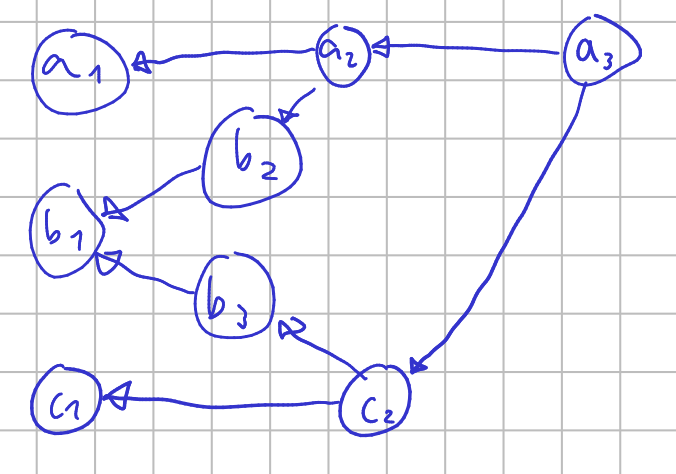
\includegraphics[width=.5\textwidth]{figures/fork_scenario_1.png}
%     \caption{An example scenario of a fork in a message graph, where $a_3$ could be considered invalid}
%     \label{fig:fork_scenario_1}
% \end{figure}
% \begin{figure}[h]
%     \centering
%     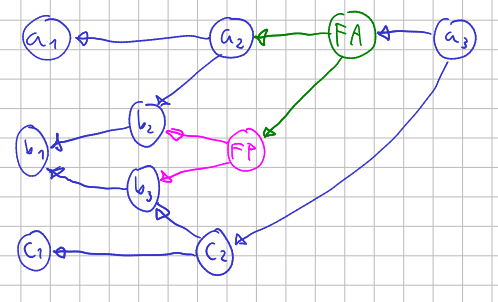
\includegraphics[width=.5\textwidth]{figures/fork_scenario_1_fixed.png}
%     \caption{The example message graph of Figure \ref{fig:fork_scenario_1} but where $a$ behaves correctly}
%     \label{fig:fork_scenario_1_fixed}
% \end{figure}
% Here is an invariant that arises naturally: for a message $M$, the induced subgraph of its dependencies only has forks that were acknowledged by author $M_\textit{author}$, i.e.

\section{Signature Verification}
As far as we know, there is no way to get the signer of a commit using a format placeholder in the Git CLI. We can only check that a signature is valid, but not that $M_\emph{author}$ is the creator of $M_\emph{signature}$, which makes this check alone useless. To remedy this, we run the \texttt{git show} command for each commit that has a valid signature (based on the signature validity retrieved with the format placeholder \texttt{\%G?}) with the \texttt{--format=raw} option, which prints the raw commit info including the base64 encoding of the signature, from which we can extract the signer and check that it matches $M_\emph{author}$.

\todo{add git command summary}

\chapter{Evaluation}
\label{sec:evaluation}
When evaluating our design, we focused on two metrics. The first was performance of the verification algorithm and the second was efficiency of storage.
Concerning performance, there are two things we are interested in: how is the scaling behaviour as we increase the number of messages we verify? and how does the optimization mentioned in Section~\ref{sec:impl-verification-alg} affect the runtime?
Concerning storage, we compare how much less storage on the hard disk our design uses by storing account data in the message of a commit compared to storing the data in the tree and blob objects as in the delta-GOC-Ledger by Heisch \cite{delta-goc-ledger-heisch}.

\section{Methodology}
\subsection{Generating baseline Repository}
\label{sec:base-repo}
To get a baseline performance and storage measurement, we created a benchmark that contains random transactions between a fixed number of authors, where the number of transactions per author follows a heavy-tailed distribution (a Pareto-distribution in our case), as it often does in real-world scenarios \cite{bitcoin-distribution-transactions}. In the performance benchmark, the number of simulated transactions is varied to indicate asymptotic scaling of the runtime of different parts of the code. Additionally there is an acknowledgement delay, meaning tokens that were given don't get acknowledged immediately. However the messages are assumed to always be replicated instantly, meaning all the participants know about the latest messages when creating a new one. Note that this doesn't mean that messages are totally ordered, since the immediate dependencies of an account message are only of the relevant participants of a transaction.

\subsection{Generating Repository including Forks}
\todo{if there is time: specify a more general way to generate transaction data including forks and byzantine acknowledgements}

\subsection{Performance benchmark}
We generate repositories with the number of messages varying from 300 to 900 with a step size of 300 and the number of authors fixed at 30.
To measure the runtime of different parts of the code, we use the \texttt{perf\_counter} function from the \texttt{time} module in the standard library of python \cite{pythonPerfCounterNs}.
We split the code into various non-overlapping sections that get measured individually and get a label in the plot.
The Code is then run with and without the optimization mentioned in section \ref{sec:impl-verification-alg}.

\subsection{Storage Bench: Comparison of storage methods}
We take the simulation described in section \ref{sec:base-repo} and use it to create repositories with the same encoded transactions, the number of messages being 1000 and the number of authors being 30. The only difference between them is how the messages are stored and how many dependencies each message has.

In the encoding labelled ``Message'', the account data is stored as described in \ref{sec:syntax-of-msgs}. In the ``Tree'' encoding, the account data is stored as nested tree and blob objects, as described by Heisch \cite{delta-goc-ledger-heisch}. More concretely json objects in our encoding map to tree objects and GOCs are represented as blob objects which contain the bytes that represent the number they store (using the functions \verb|int.to_bytes| and \verb|int.from_bytes| in the standard library of python to encode and decode respectively).

The number of dependencies is also varied. By ``Extra Deps.'' we mean that a message stores a reference for each other author pointing to the last known message that the creator knew about, as opposed to just the last messages of the authors that appear in the transaction.

To measure the size of the generated repositories, we use the unix command \texttt{du} (disk usage) on the corresponding \texttt{.git} directory with the flag \texttt{-s} to get the total storage size this directory takes up. This value is in the column ``Effective Size''. The command \texttt{git gc} is used to compress the git repository. We measure each size before and after running this command which correspond to the columns ``Uncompressed'' and ``Compressed'' respectively.

\subsection{Relevant Specs of System}
The Benchmarks are run on a Lenovo ThinkPad X13 2-in-1 with the specs shown in Table~\ref{tab:specs}.
One important thing to note when using WSL2 as a virtual machine is that the performance is degraded significantly when accessing files from a mounted directory \cite{wsl2FilesystemPerf}. We run the benchmark with associated data in the home directory, where this issue doesn't arise.
\begin{table}
\centering
\begin{tabular}{|l|p{6cm}|}
    \hline
    OS & WSL version 2.7.10.0 running Ubuntu 24.04.4 LTS with Microsoft Windows 11 Pro as host OS\\ \hline
    System Type & x64-based PC\\ \hline
    Processor & Intel(R) Core(TM) Ultra 5 125U, 1300 Mhz, 12 Cores, 14 Logical Processors\\ \hline
    Installed Physical Memory (RAM) & 16.0 GB\\ \hline
    Git version & 2.43.0 \\ \hline
\end{tabular}
\caption{relevant specs of the hard- and software used to perform benchmarks}
\label{tab:specs}
\end{table}

\section{Results}
\label{sec:results}
\subsection{Performance of Verification Algorithm on baseline repository}
\label{sec:results:perf-baseline}
\begin{figure}
    \centering
    \begin{subfigure}{0.49\textwidth}
        \centering
        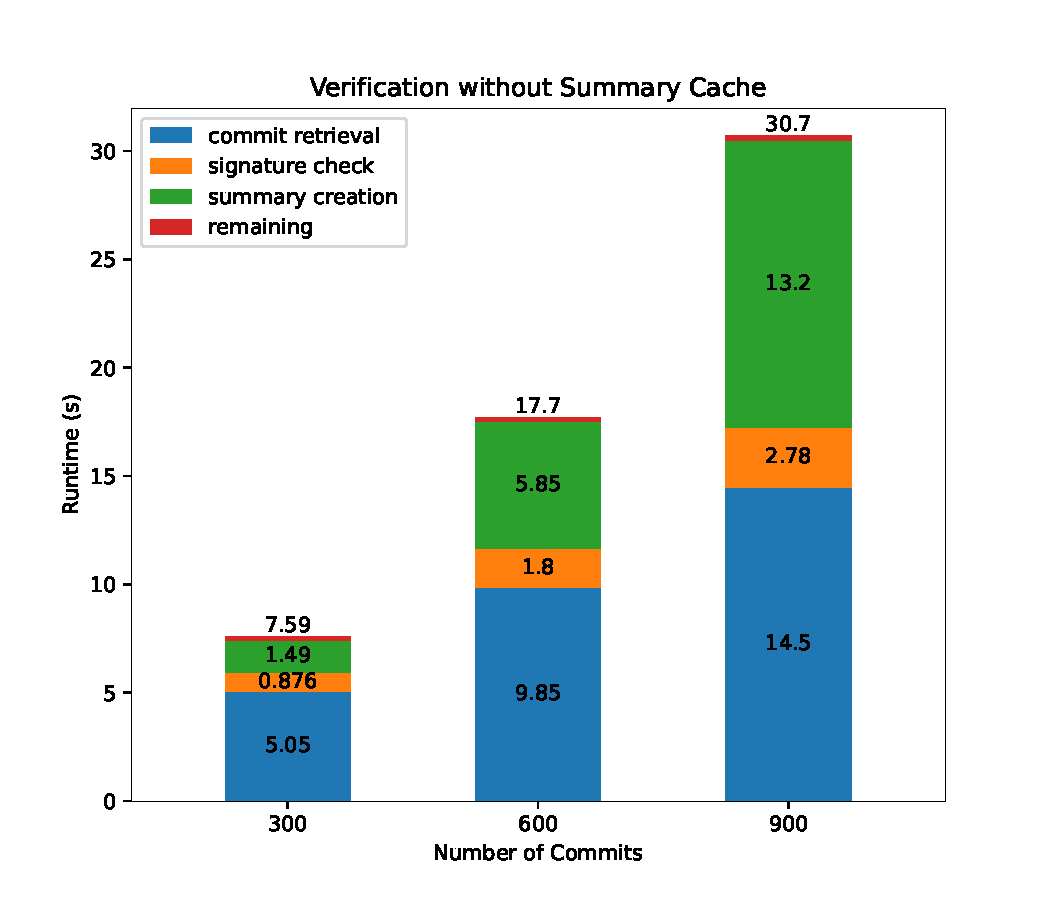
\includegraphics[page=1,width=1.\textwidth]{figures/Verification without Summary Cacheplot.pdf}
    \end{subfigure}
    \begin{subfigure}{0.49\textwidth}
        \centering
        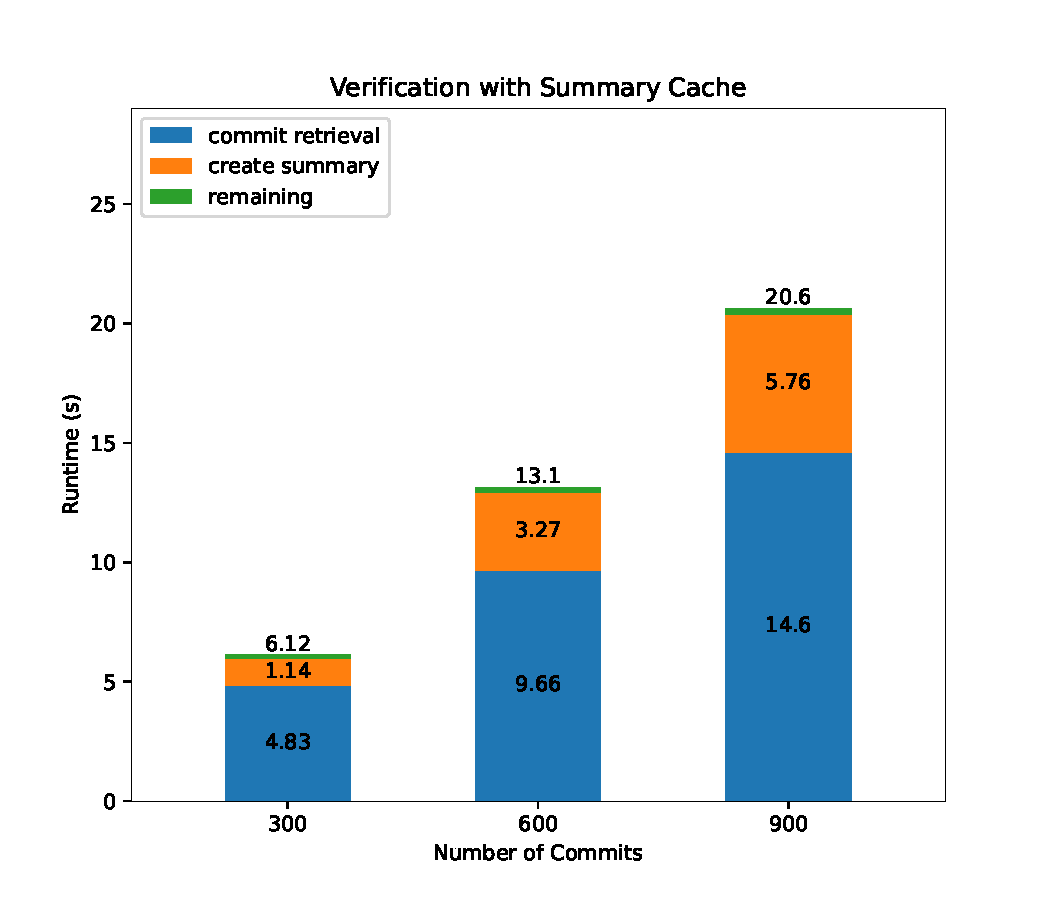
\includegraphics[page=1,width=1.\textwidth]{figures/Verification with Summary Cacheplot.pdf}
    \end{subfigure}
    \caption{Performance measurements on baseline repository with and without the summary cache optimization}
    \label{fig:perf-result}
\end{figure}

The results of the performance benchmark done on the baseline repository are shown in figure \ref{fig:perf-result}. The sections corresponding to ``commit retrieval'', ``signature check'', ``summary creation'' and ``remaining'' are the total time spent checking the signatures of commits, retrieving all the commits initially, creating the summary and the remaining time not measured by any of the other ones, respectively. Most of the remaining time will be taken up by checking the invariants given the summary data structure.
If we take a look at the verification algorithm without the summary cache optimization, we see that the total running time (top of the bars) increases more than proportionally with respect to the number of commits. The section that is responsible for this scaling is mostly ``create summary''. However if we take a look at the graph with the summary cache optimization, we see that ``create summary'' is no longer that big of a part of the total runtime and increases less quickly.

\subsubsection{Discussion}
The reason ``summary creation'' is the biggest part of the time besides ``commit retrieval'', is because we use subprocesses to recreate the summary, which happens for each commit, even with the summary cache optimization.

If we take a look at the graph without the summary cache optimization, we see that the label ``summary creation'' scales quite quickly. This is because for each commit we recreate the summary from scratch, which means we have to look at the whole causal history, which comprises only of commits that were already visited. This is a lot of unnecessary work and intuitively leads to an asymptotic scaling which is roughly quadratic in terms of the number of commits.

Once the summary cache optimization is applied, we see that this scaling is less aggressive, yet still not proportional to the number of commits. This is not because we occasionally miss the cache: since there are no forks, cache misses are impossible (except for the initial messages of an author). We believe this scaling is this way because the more commits we have visited previously, even if we get a summary cache hit, the more additional commits may need to be traversed to create the summary.

\subsection{Storage Bench}
When measuring the size of the generated git repositories, we get the result shown in Table~\ref{tab:storage-res}.
We see that the compressed versions of the tree encoding are less than 10\% of their uncompressed versions, while the compressed versions of the message encoding take up more than 20\% (21\% and 23\%) of the uncompressed ones.
Additionally, we see the repositories without the extra dependencies are between about 78\% and 92\% of their corresponding repository with the extra dependencies.
We also see that encoding the data as messages and storing no extra dependencies (our approach) uses about 69\% of the space that uses the tree encoding with extra dependencies (proposed by Heisch \cite{delta-goc-ledger-heisch}) uses when looking at the effective size after compressing the files. The difference is bigger if we take a look at the effective size before compressing: then our approach only uses about 29\% of the approach proposed by Heisch.

% \begin{table}
%     \centering
%     \begin{tabular}{|l|l|l|l|l|l|}
%         \hline
%         \multicolumn{2}{|c|}{\textbf{Method}} & \multicolumn{2}{|c|}{\textbf{Real Size}} & \multicolumn{2}{|c|}{\textbf{Apparent Size}} \\ \hline
%         \textbf{Encoding} & \textbf{Extra Deps.} & \textbf{C} & \textbf{U} &\textbf{C} & \textbf{U} \\ \hline
%         Tree              & Yes                               & 2268                & 23228                 & 1300               &7907  \\ \hline
%         Tree              & No                                & 2044                & 21392                 & 1079               &6114  \\ \hline
%         Message           & Yes                               & 1860                & 8624                  & 896                &2483  \\ \hline
%         Message           & No                                & 1572                & 6772                  & 617                &673   \\ \hline
%     \end{tabular}
%     \caption{Result of storage benchmark, numbers in kB. \textbf{C} and \textbf{U} correspond to compressed and uncompressed respectively.}
%     \label{tab:storage-res}
% \end{table}
\begin{table}
    \centering
    \begin{tabular}{|l|l|l|l|}
        \hline
        \multicolumn{2}{|c|}{\textbf{Method}} & \multicolumn{2}{|c|}{\textbf{Effective Size}} \\ \hline
        \textbf{Encoding} & \textbf{Extra Deps.} & \textbf{Compressed} & \textbf{Uncompressed} \\ \hline
        Tree              & Yes                               & 2268                & 23228                 \\ \hline
        Tree              & No                                & 2044                & 21392                \\ \hline
        Message           & Yes                               & 1860                & 8624                 \\ \hline
        Message           & No                                & 1572                & 6772                 \\ \hline
    \end{tabular}
    \caption{Result of storage benchmark, numbers in kB.}
    \label{tab:storage-res}
\end{table}
\subsubsection{Discussion}
We see that the space saved by encoding account data in the message of the commit is significant, especially when looking at the uncompressed version of the repositories.
This is the case, because there are a lot of extra objects that need to be stored in the case of the tree encoding: for each GOC value, we store a blob which is identified with a 32-byte SHA256 value. This value has to be stored in the tree objects. One advantage that the tree encoding could have is deduplication of equivalent values. However by the time deduplication would be effective, i.e. if the number of bytes stored in them is greater than the identifier (greater than 32 bytes), the numbers stored in the objects are unlikely to be equivalent, rendering deduplication unapplicable.

However the tree encoding gets compressed more effectively than the message encoding. We think this is the case because git packs the tree and blob files into files without explicitly storing the identifiers of these objects. Still, our encoding is more effective at storing the data in the benchmark, even after compression.

\chapter{Related Work}
The design of the delta-GOC-Ledger, as well as of the 2P-BFT-Log was taken directly from the Masters Thesis of Heisch \cite{delta-goc-ledger-heisch} and the Paper of Lavoie \cite{2p-bft-log} respectively. What was attempted in this report was to unify the two designs. To do this, we took inspiration from the Blocklace paper by Almeida et al. \cite{blocklace-crdt}. Additionally, none of the papers mentioned above described a verification procedure, which we partly specified and implemented. We also extended the designs by limiting the number of dependencies per transaction and adding a new message type.

\chapter{Conclusion}
In this report, we specified new invariants that need to be considered when implementing the $\delta$-GOC-Ledger over such a byzantine fault tolerant log and how they interact. We then specified and implemented an algorithm that verifies these invariants. Additionally, we implemented an optimization that reduced the rate of increase of the running time with respect to the number of commits significantly. We also adapted the encoding of the account data in commit objects from the originally proposed design of Heisch and were able to achieve about a 70\% reduction in storage space when uncompressed and about a reduction of 30\% when compressed, while also being easier to retrieve using the Git CLI.

\subsection{Future Work}
Considering the design of the algorithm, there are some things to be done; the verification algorithm still has to be extended to include invariant \var{F4}, which we argue should guarantee byzantine repellance, as defined in the Blocklace paper \cite{blocklace-crdt}. Furthermore, the design of our algorithm is not proven to verify the mentioned invariants.
Additionally, we have to keep track of an increasing amount of state as more commits get verified (for example $C_\emph{msg}$ and $F_\emph{valid}$). This could be solved by using some sort of reference counting technique to drop the entries in these sets that don't get referenced by new commits.

Considering the implementation of the algorithm, we think the creation of the summary can be improved by a lot if the commit traversal ran in the same process as the verification algorithm, rather than calling the Git CLI through the subprocess module. This is possible, because at the time of creating a summary, we have all the data that is needed to traverse the commit graph in $C_\emph{msg}$.

Considering the performance evaluation of our algorithm, we only took a look at a very basic benchmark that does not include byzantine behaviour. To remedy this, a benchmark would have to be created that includes forks and other byzantine behaviour.

Considering the encoding of delta accounts as commit messages, instead of using json serialization, we could use a more efficient custom format.

Considering the design of the invariants, the problem of double spending still persists and has to be solved by designing a system that prevents correct replicas from losing tokens or tokens being created out of thin air.
